% Prof. Dr. Ausberto S. Castro Vera
% UENF - CCT - LCMAT - Curso de Ci\^{e}ncia da Computa\c{c}\~{a}o
% Campos, RJ,  2021
% Disciplina: Paradigmas de Linguagens de Programa\c{c}\~{a}o
% Aluno:


\chapterimage{ScalaH} % Chapter heading image
\chapter{Conclus\~{o}es}
\begin{quote}
    Diante de tudo que aprendemos durante essa jornada. Nos encontramos aqui, mais fortes e mais sábios.
    Mesmo com os problemas enfrentados na hora de executar muitos dos códigos apresentados, versão do compilador desatualizada, dificuldades com o entendimento da linguagem Scala.
    Sabendo que, este livro foi produzido pensando em ser uma forma rápida de recapitular conceitos essenciais na hora de programar em uma das suas linguagens favoritas; Scala. Dessa forma, foi alcançado o objetivo desejado de entregar algo que possibilita um aprendizado rápido de umas das linguagens de programação mais usadas do mercado. Abrindo portas para programação Web, Computação distribuída, Data Science, programação funcional (cujo não cobrimos durante este livro) etc.
    Sendo assim, é altamente recomendado que no futuro venha aprender os conceitos da programação funcional na linguagem de programação Scala. Esse novo paradigma de programação proporcionará novas formas de enxergar os problemas que encontrará durante a sua carreira na academia e no mercado de trabalho.

    Nossa jornada não termina aqui. Deixo uma recomendação de um livro que trabalha a fundamentar os conceitos de programação funcional e de programação orientada a objeto. Segue abaixo o material recomendado para continuar os estudos em Scala.
    \begin{figure}[H]
        \begin{center}
            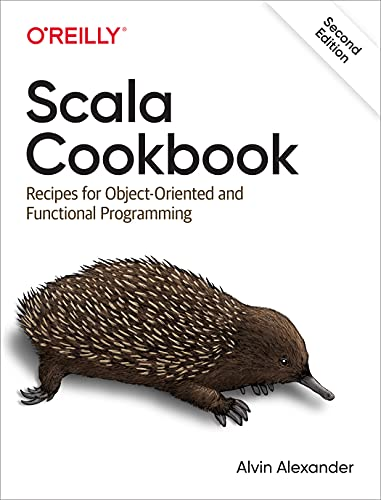
\includegraphics[width=7cm]{paradigm}
            \caption{Scala Cookbook: Recipes for Object-Oriented and Functional Programming} \label{ling2}
            {\tiny \sf Fonte: Amazon Serviços de Varejo do Brasil Ltda.  }
        \end{center}
    \end{figure}
\end{quote}
